\section{Empirijski podaci o površinama izmjene}\label{sec:empirija}

\izjava{E1}{Pluća sisavaca: alveolarna i kapilarna površina skaliraju s $M^{0{,}92}$ (95~\% IP 0,87–0,97). Morfometrijski difuzijski kapacitet $D_{LO_2}$ skalira s $M^{0{,}95}$ (0,89–1,01) u podskupu iz teksta, odnosno s $M^{0{,}99}$ u sažetku. $\dot V_{O_2\max}$ skalira s $M^{0{,}79}$, a volumen kapilara približno s $M^{1}$. (Gehr i sur. 1981) \pouzd{puni tekst (OCR); sažetak}}
\izjava{E2}{Mišić sisavaca: $\dot V_{O_2\max}\propto M^{0{,}872\pm0{,}029}$ (34 vrste). $\dot V_{O_2\max}$ je linearno povezan s ukupnim volumenom mitohondrija i kapilara u mišićima, pa te strukture skaliraju približno kao $M^{0{,}87}$ ako ta linearna veza vrijedi za svih 34 vrste. Izravno izmjereni eksponenti struktura (podskup od 11 vrsta) navedeni su u E10. (Weibel i Hoppeler 2005) \pouzd{puni tekst za $\dot V_{O_2\max}$; izvedeno za strukture}}
\izjava{E3}{Škrge slatkovodnih riba: eksponenti površine škrga kreću se od 0,36 do 1,13, sa srednjom vrijednošću 0,76. (Palzenberger i Pohla 1992) \pouzd{sažetak}}
\izjava{E4}{Šaran (\emph{Cyprinus carpio}): nagib površine škrga je 7,066 u prelarve, 1,222 u postlarve (do 0,2~g) i 0,794 između 0,2 i 2250~g. Površina tijela skalira s 0,52–0,72. (Oikawa i Itazawa 1985) \pouzd{puni tekst}}
\izjava{E5}{Chinook losos: pri izlijeganju koža čini oko 96~\% površine izmjene, a škrge je prestižu tek pri 2,5–4~g. (Rombough i Moroz 1990) \pouzd{puni tekst}}
\izjava{E6}{Obrtaj ugljika i dušika u cijelom tijelu i mišiću skalira kao $M^{-0{,}19}$ i ovisi o temperaturi; splanhnička tkiva (probavni sustav, utroba) ne slijede taj odnos (Thomas i Crowther 2015). Ugradnja $^{13}$C u krv ptica skalira približno kao $M^{-1/4}$ (Carleton i Martínez del Rio 2005). \pouzd{sažetak}}
\zaalfa{ako je specifična brzina izmjene $\propto V^{\alpha-1}$ (P3) i $V\propto M$, onda $M^{-0{,}19}$ daje $\alpha\approx0{,}81$, a $M^{-1/4}$ daje $\alpha\approx0{,}75$ \pouzd{izvedeno}. Ovo je samo gruba provjera, jer obrtaj u cijelom tijelu miješa obrtaj proteina i razrjeđenje rastom, a riječ je o interspecifičnim podacima.}
\izjava{E7}{Planarije: Kleiberovo skaliranje metabolizma ne dolazi od pada metabolizma po stanici, nego od toga što masa po stanici raste s veličinom tijela. Uzrok je pohrana energije koja ovisi o veličini. (Thommen i sur. 2019) \pouzd{sažetak}}
\izjava{E8}{Planarije: tijekom rasta crijevo dobiva nove grane duž cijele uzdužne osi, preoblikovanjem postojećeg crijeva. Broj grana dakle raste s veličinom, ali eksponent nije objavljen. (Forsthoefel, Park i Newmark 2011) \pouzd{sažetak}}
\zaalfa{kod planarija i eksponent asimilacije $a$ i $\alpha$ mogu biti iznad $2/3$. Prema P2 gustoća spremišta otkriva samo razliku $a-\alpha$, pa planarije zahtijevaju neovisno mjerenje unosa hrane.}
\izjava{E9}{Mrežnica čovjeka: na digitaliziranim kolažima fluoresceinskih angiograma fraktalna dimenzija arterijskog stabla je $1{,}63\pm0{,}05$, a venskog $1{,}71\pm0{,}07$, u skladu s dimenzijom rasta ograničenog difuzijom (DLA) od $1{,}68\pm0{,}05$ (Mainster 1990). Na 2-D slikama normalnih i tumorskih krvožilnih mreža razlikuju se tri klase skaliranja: normalne arterijsko-venske mreže skaliraju kao rast ograničen difuzijom, normalne kapilarne mreže su kompaktne strukture, a tumorske mreže skaliraju kao perkolacijski klasteri (Gazit i sur. 1995). \pouzd{sažetak}}
\zaalfa{prema P6 dimenzije stabala 1,63–1,71 daju $\alpha_{2D}=D/2=0{,}815$–$0{,}855$, a kompaktna kapilarna mreža ($D=2$ u ravnini) daje $\alpha_{2D}=1$ \pouzd{izvedeno}. Isto tkivo daje dva različita odgovora, ovisno o tome mjeri li se stablo ili kapilarno korito. Za $\alpha$ je mjerodavno korito (T16, H4).}
\izjava{E10}{Mišić sisavaca, morfometrija cijelog tijela u 11 vrsta (20~g–450~kg): ukupni volumen kapilara lokomotornih mišića skalira kao $M^{0{,}984}$ (95~\% IP 0,909–1,056), ukupni volumen mitohondrija kao $M^{0{,}956}$ (0,846–1,066), a $\dot V_{O_2\max}$ istih vrsta kao $M^{0{,}962}$ (0,829–1,096). Masa mišića skalira kao $M^{1{,}01}$, a promjer kapilara gotovo ne ovisi o masi tijela ($\propto M^{0{,}01}$) (Weibel i Hoppeler 2005). Kod 25 afričkih vrsta (0,4–251~kg) broj kapilara po presjeku vlakna raste s volumnom gustoćom mitohondrija, ali uz velik rasap, pa sam broj kapilara nije dovoljan opis opskrbe (Hoppeler i sur. 1981b). Unutar jedne životinje volumna gustoća mitohondrija u vlaknima iznosi 10–12~\% u ošitu i 1–6~\% u ostalim mišićima (Hoppeler i sur. 1981a). \pouzd{puni tekst za Weibel i Hoppeler 2005; sažetak za Hoppeler i sur. 1981a, b}}
\zaalfa{volumen kapilara po volumenu mišića skalira kao $M^{0{,}984-1{,}01}\approx M^{-0{,}03}$, tj. gustoća kapilara gotovo ne ovisi o veličini tijela. Uz promjer $d\propto M^{0{,}01}$ ukupna površina kapilara je $S\propto V(c)/d\propto M^{0{,}97}$, a površinska gustoća $S_V\propto M^{-0{,}04}$. Uz $S_V\propto V^{\alpha-1}$ i $V\propto M$ to daje morfometrijski $\alpha\approx0{,}97$, odnosno približno 0,90–1,05 iz intervala za volumen kapilara \pouzd{izvedeno}. Tri ograde: podaci su interspecifični, a $\alpha$ je ontogenetski eksponent; kapilare prate vršnu potražnju za kisikom (T15), pa je ovo prior i gornja granica za energijski $\alpha$; gustoća se razlikuje među mišićima, a takve razlike prema H3 idu u $\beta$.}

\begin{figure}[ht]
\centering
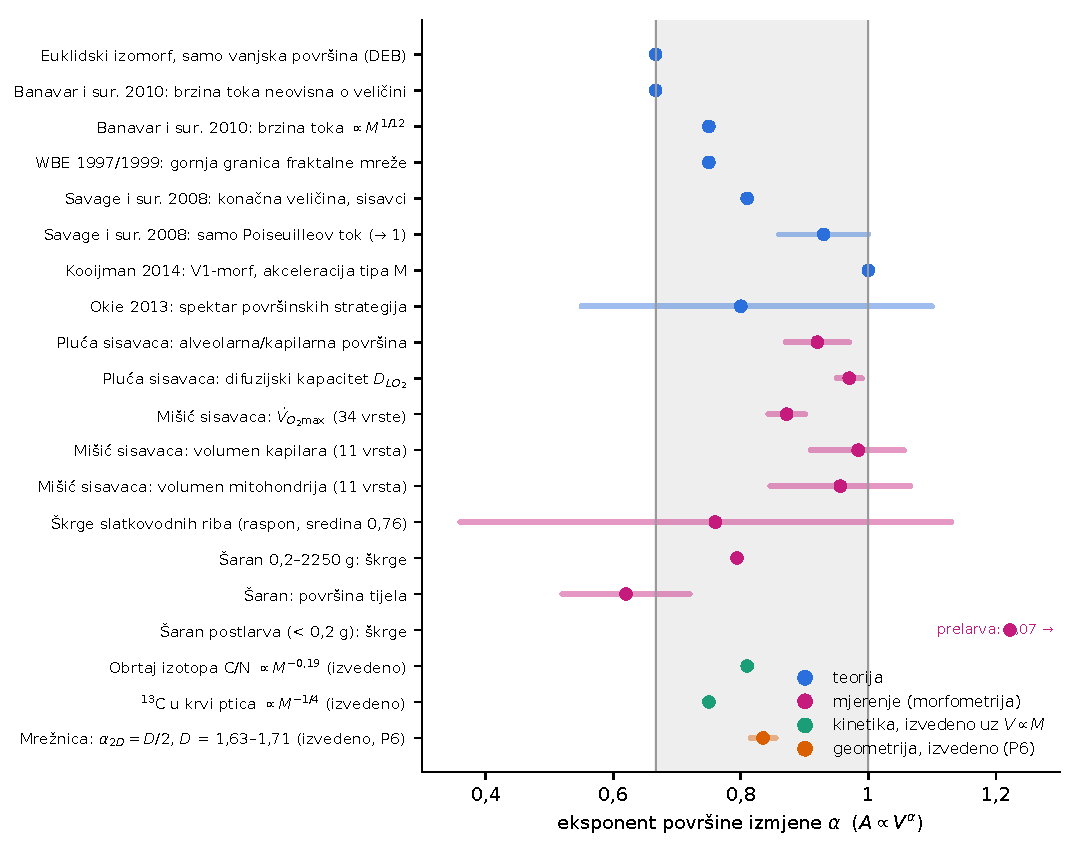
\includegraphics[width=\linewidth]{figures/fig_atlas.pdf}
\caption{Atlas eksponenata važnih za $\alpha$. Siva zona je radni raspon $2/3$–$1$. Plavo: teorijska predviđanja (T3, T8–T11). Ljubičasto: morfometrijska mjerenja s rasponom ili intervalom pouzdanosti (E1–E4). Zeleno: eksponenti izvedeni iz kinetike obrtaja uz $V\propto M$ (E6). Nagib škrga u prelarve šarana (7,07) izlazi izvan skale.}
\label{fig:atlas}
\end{figure}

\begin{kljucno}[Tri pouke iz podataka]
\begin{enumerate}[leftmargin=1.4em]
\item \textbf{Strukture za izmjenu kod sisavaca skaliraju s 0,87–0,99}, strmije od WBE granice od $3/4$ (E1, E2, E10, T8). Gustoća kapilara u mišiću gotovo ne ovisi o veličini tijela (E10). Prate \emph{vršnu} potražnju ($\dot V_{O_2\max}\propto M^{0{,}79}$–$M^{0{,}87}$), a ne bazalni metabolizam. Morfometrija je stoga gornja granica i prior za $\alpha$, a ne procjena.
\item \textbf{$\alpha$ ovisi o životnom stadiju.} Kod šarana nagib škrga pada s 7,07 na 1,22 i zatim na 0,79 (E4). Kod lososa se izmjena seli s kože na škrge (E5). Jedan $\alpha$ za cijeli život je pojednostavljenje.
\item \textbf{$\alpha$ ovisi o vrsti.} Raspon eksponenata škrga među slatkovodnim ribama je 0,36–1,13 (E3). Univerzalna vrijednost ne postoji, što je u skladu s hipotezom H6 o $\alpha$ kao svojstvu vrste ili klade.
\end{enumerate}
\end{kljucno}
